\documentclass[12pt,a4paper,openright]{book}

\usepackage{ThesisStyle} %样式模板

%\usepackage{showframe} %显示文档框架,用于检查内容是否超出页面布局

\newacronym{IoT}{IoT}{Internet of Things}
\newacronym{CEO}{CEO}{chief executive officer}
\newacronym[sort=pmf]{pmf}{\emph{pmf}}{probability mass function}
\newacronym{iid}{i.i.d.}{independent and identically distributed} %定义缩略语
\newglossaryentry{t}{ %符号ID
	sort=t, %以该字符串为依据排序
	type=symbols, %术语类型为符号
	name={$t$}, %符号名称
	description={time index} %符号描述
}
\glsadd{t} %将该ID对应的符号加入到列表中

\newglossaryentry{C}{
	sort=C,
	type=symbols,
	name={$C(\cdot)$},
	description={the Shannon capacity using Gaussian codebook}
}
\glsadd{C}

\newglossaryentry{delta}{
	sort=z_delta,
	type=symbols,
	name={$\delta(\epsilon)$},
	description={a function of $\epsilon$ that tends to zero as  $\epsilon \to 0$}
}
\glsadd{delta}
 %定义符号

\begin{document}

\pagestyle{empty}
\begin{center}
修士論文 \\
\vspace{80pt}
〇〇〇〇〇題目〇〇〇〇〇\\
\vspace{80pt}
1710000 % 学生番号
\quad
〇〇氏名〇〇\\
\vspace{100pt}
\begin{tabular}{rl}
主指導教員 & 〇〇 〇〇\\
審査委員主査 & 〇〇 〇〇\\
審査委員 & 〇〇 〇〇\\
& 〇〇 〇〇\\
& 〇〇 〇〇
\end{tabular}\\
\vspace{90pt}
北陸先端科学技術大学院大学\\
先端科学技術研究科\\ % または情報科学研究科
(情報科学)\\ %取得希望学位
\vspace{90pt}
平成31年2月\\ % 提出年月
\end{center}
\cleardoublepage %封面

\pagenumbering{Roman} %页码使用大写罗马数字
\titleStyleCenter

%%%%%%%%%%%%%%%%摘要和致谢%%%%%%%%%%%%%%%%%%%%%%%
\newcommand{\AbstractName}{Abstract}
\chapter*{\AbstractName}
\addcontentsline{toc}{chapter}{\AbstractName}

Write abstract here.

\textbf{Keywords:} Keyword1, keyword2, keywor3.
\newcommand{\AckName}{Acknowledgment} %致谢名称
\chapter*{\AckName}
\addcontentsline{toc}{chapter}{\AckName}
%%%%%%%%%%%%%%%%%%%%%%%%%%%%%%%%%%%%%%%%%%%%%%%%%%%%%%%

Write acknowledgment here.




%%%%%%%%%%%%%%%%摘要和致谢end%%%%%%%%%%%%%%%%%%%%

\titleStyleList

%%%%%%%%%%%%%%%%图片、表格、术语列表%%%%%%%%%%%%%%%
\renewcommand{\acronymname}{List of Abbreviations} %设置缩写列表名称
\renewcommand{\symbolname}{List of Symbols} %设置符号列表名称

\printglossary[type=\acronymtype] %插入缩略语列表
\setglossarystyle{clong} %设置列表风格,首字母不大写
\printglossary[type=symbols] %插入符号列表
\glsresetall %重置术语列表的引用

\listoffigures %插入图片列表
\listoftables %插入表格列表
\tableofcontents %插入目录
%%%%%%%%%%%%%%%%图片、表格、术语列表end%%%%%%%%%%%%

\cleardoublepage
\pagenumbering{arabic} %正文页码使用阿拉伯数字
\setcounter{page}{1} %正文页码从1开始

%%%%%%%%%%%%%%%%%正文章节%%%%%%%%%%%%%%%%%%%%%%%%
\titleStyleChapter
\chapter{Introduction}

\section{Section}
\subsection{Subsection}
\subsubsection{Subsubsection}


\ref{cha:conclusion}

\ref{app:example}

\section{Figures}

\begin{figure}[ht]
\centering 

\includegraphics[scale=0.4]{Figures/jpgFigure.jpg}
\caption{JPG figure title.}
\label{fig:jpgFigure}
\end{figure}

\begin{figure}[ht]
\centering 
\subfigure[PDF figure title.]{
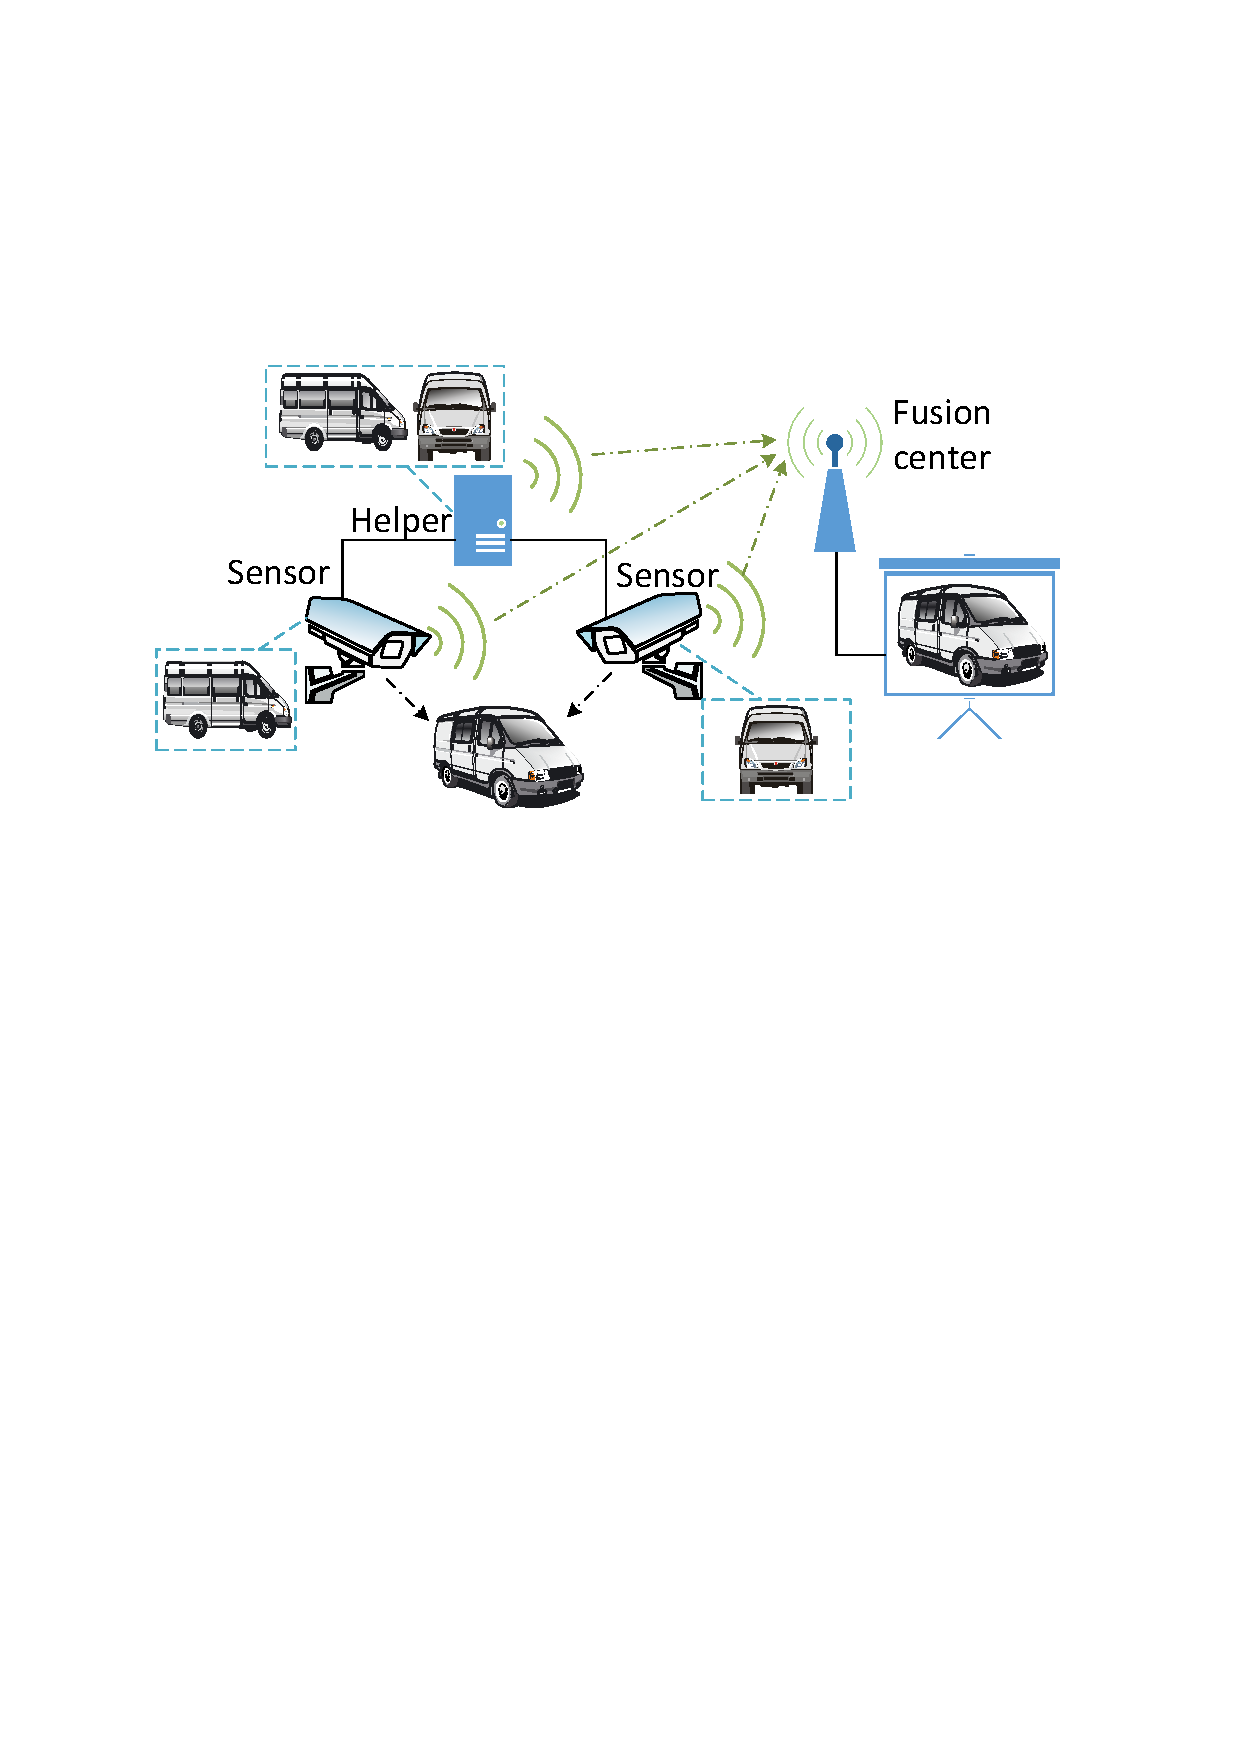
\includegraphics[height=4cm]{Figures/pdfFigure.pdf}
\label{fig:pdfFigure}
}
\subfigure[EPS figure title.]{
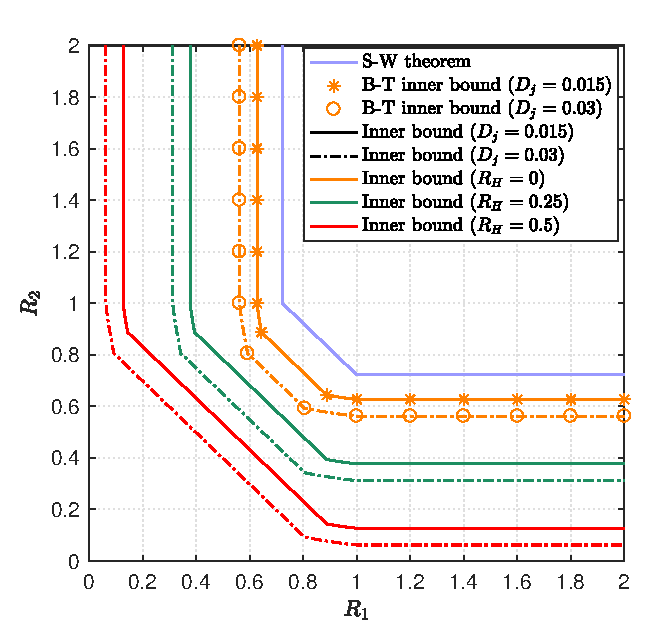
\includegraphics[height=4cm]{Figures/epsFigure.eps}
\label{fig:epsFigure}
}
\caption{Subfigure Examples.}
\label{fig:examples}
\end{figure}

\fref{fig:jpgFigure}

\fref{fig:examples}

\fref{fig:epsFigure}

\section{Tables}
\begin{table}[ht]
\centering
\begin{tabular}{r|rr}
& a & b\\ 
\hline
1& 0.25 & 0.33\\
2& 0.75 & 0.66\\
\end{tabular}
\caption{Caption of the table}\label{table:example}
\end{table}

\tref{table:example}

\section{Equations}

\begin{equation}
x = \frac{-b \pm \sqrt{b^2-4ac}}{2a}. \label{eq:example}
\end{equation}

\begin{align}
x^2 &= -(2x +1) \\
x^2 &= -2x -1 \nonumber\\
x^2+2x +1 &= 0 \label{eq:example2}\\
(x+1)^2 &=0 \label{eq:example3}.
\end{align}

\eqref{eq:example3}

\eqsref{eq:example}{eq:example2}

\section{Abbreviations and Symbols}
\gls{iid}


\Gls{CEO}


\glspl{CEO}

\gls{IoT}


\Glspl{pmf}

\section{Citations}
\cite{berger1978multiterminal}

\cite{berrou1996near,shannon1959coding,el2011network,mp3standard}

\cite{el2011network,berger1978multiterminal}

\cite{Tung1978multiterminal}

\section{Algorithms}
\begin{algorithm}
\caption{An Example}
\label{alg:example}
\begin{algorithmic}
\REQUIRE {$x$, $n$} 
\ENSURE {$y$}
\STATE {set $y=1$;} 

\IF	{$n==0$} 
	\STATE {set $y=1$;} 
\ELSIF {$n>0$} 	
	\FOR {$i=1$ \TO $n$} 		
		\STATE {set $y = y \times x$;} 
	\ENDFOR
\ELSE
	\FOR {$i=n$ \TO $-1$} 		
		\STATE {set $y = y \div x$;} 
	\ENDFOR 
\ENDIF
\end{algorithmic}
\end{algorithm}

\algref{alg:example}

\section{Codes}
\begin{lstlisting}[
	language=C++,
	title={No Number Title},
	label={code:example} ] % 设置语言、标题、标签
%以下插入代码,必须隔一行空行

int main(){
	for(int i=0; i<3; i++){
		cout<<i<<endl;
	}
	return 0;
}
\end{lstlisting}

\lstinputlisting[
	language=TeX,
	caption={Input Code from File},
	label={code:input}]
	{Chapters/Conclusion.tex} %从文件中插入代码

\coderef{code:input}

\chapter{Conclusion}\label{cha:conclusion}

This thesis ...


%%%%%%%%%%%%%%%%%正文章节end%%%%%%%%%%%%%%%%%%%%

\appendix
%\FistAppdfalse %注释掉\FistAppdfalse,则会在目录中第一个附录之前,额外增加一行“附录”链接
%%%%%%%%%%%%%%%%附录%%%%%%%%%%%%%%%%%%%
\chapter{Example}\label{app:example}

Number test in Appendices.

\begin{equation}
x(i)=x^i, \textrm{ for } i=\{1,2,\cdots,n\} \label{eq:app1}
\end{equation}
\eqref{eq:app1}

\tref{table:app}

\begin{table}[ht]
\centering
\begin{tabular}{c|c}
\hline
\bfseries Parameter & \bfseries Value \\
\hline
\hline
Block length & $10000$ bits \\
\hline
Number of Blocks & $1000$ \\
\hline
\end{tabular}
\caption{Table in Appendix}\label{table:app}
\end{table}

\chapter{Code Example}\label{app:code}

\lstinputlisting[
	language=Matlab,]
	{Appendices/CodeExample.m} %从文件中插入代码

%%%%%%%%%%%%%%%%附录end%%%%%%%%%%%%%%%%%%%
\titleStyleList


%%%%%%%%%%%%%%%%参考文献%%%%%%%%%%%%%%%%%%%
\renewcommand{\bibname}{References} %设置参考文献标题
\bibliographystyle{IEEEtran} %参考文献样式
\bibliography{myReference} %参考文献bib文件
%%%%%%%%%%%%%%%%参考文献end%%%%%%%%%%%%%%%%%%%

%%%%%%%%%%%%%%%%%学术成果end%%%%%%%%%%%%%%%%%%%%
\newcommand{\PubName}{Publications}
\chapter*{\PubName}
\addcontentsline{toc}{chapter}{\PubName}
\begin{publication}
\item
{ISO/IEC International Standard 11172-3}, ``Coding of moving pictures and
  associated audio for digital storage media at up to about 15 {M}bit/s -
  {Part3}: {Audio},'' 1993.    
\item
A.~El~Gamal and Y.-H. Kim, \emph{Network information theory}.\hskip 1em plus
  0.5em minus 0.4em\relax Cambridge, UK: Cambridge University Press, 2011.
\end{publication}


%%%%%%%%%%%%%%%%%学术成果end%%%%%%%%%%%%%%%%%%%%
\end{document}
